\documentclass{article}
\usepackage[english]{babel}
\usepackage[utf8]{inputenc}
\usepackage{fancyhdr}
\usepackage{geometry}
\usepackage{enumitem}
\usepackage{amsmath}
\usepackage{graphicx}
\usepackage{tcolorbox}
\usepackage{amssymb}
\usepackage[thinc]{esdiff}
\usepackage{float}

\geometry{letterpaper, portrait, margin=1in}
\graphicspath{ {images/} }
\pagestyle{fancy}
\fancyhf{}
\lhead{Keerthik Muruganandam}
\rhead{Yadavalli Written Work 4}

\begin{document}

\begin{enumerate}[label=\textbf{(4.\arabic*)}]


\item Integrate $\displaystyle{ \int\!p^5\ln(p)\,dp }$

We can use the formula
\[\int\!u\,dv=uv-\int\!v\,du\]
otherwise know as IBP. Using the acronym L.I.A.T.E. to pick our $u$ and $v$, our values for them are
\begin{align*}
u&=\ln(p) \\
dv &= p^5\,dp
\end{align*}
Then, we substitute our values into the IBP formula.
\begin{align*}
\int\!u\,dv &= uv-\int\!v\,du \\
&=\ln(p)\frac{p^{5+1}}{5+1}-\int\!\frac{p^{5+1}}{5+1}\cdot\frac{1}{p}\,dp \\
&=\frac{\ln(p)p^6}{6}-\int\!\frac{p^5}{6}\,dp \\
&=\frac{\ln(p)p^6}{6}-\frac{1}{6}\int\!p^5\,dp
\end{align*}
Now we should evaluate the indefinite integral with basic antiderivatives.
\begin{align*}
    \int\!p^5\,dp &= \frac{p^{5+1}}{5+1}+C \\
    &=\frac{p^6}{6}+C
\end{align*}
Substitution back into our previous expression sums as
\begin{align*}
    \frac{\ln(p)p^6}{6}-\frac{1}{6}\cdot\frac{p^6}{6}&=\frac{\ln(p)p^6}{6}-\frac{p^6}{36}
\end{align*}
Thus, our final answer is $\dfrac{\ln(p)p^6}{6}-\dfrac{p^6}{36}$.
\newline
\begin{center}
Problem 2 on next page. $\rightarrow$	
\end{center}


\newpage %%%%%%%%%%%%%%%%%%%%%%%%%%%%%%%%%%%%%%%%%%%%%%%%%%%%%%%%%%%%%%%%%%%%%%%%%%%%%%%%%%%%%%%%%%%%%%%%%%%%%%%%%%%%%%%%%%%%%%%%%%%%%%%%%%%%%%%%%%%%%%%%%%%%%%%%%%%%%%%


\item Use substitution on the integral $\displaystyle{\int\!\frac{1}{\sqrt{x+2}+x}}$ to express the integrand as a rational function, then evaluate the integral.

Let $u=\sqrt{x+2}$. Thus, $du=\dfrac{1}{2\sqrt{x+2}}\,dx$. Now, we can use algebra to apply the Substitution Rule.
\begin{align*}
    \int\!\frac{1}{\sqrt{x+2}+x}&=\int\!\frac{2\sqrt{x+2}}{2\sqrt{x+2}}\cdot\frac{1}{\sqrt{x+2}+x} \\
    &=\int\!\frac{2\sqrt{x+2}}{\sqrt{x+2}+x}\cdot\frac{dx}{2\sqrt{x+2}} \\
    &=\int\!\frac{2\sqrt{x+2}}{\sqrt{x+2}+x}\, du \\
    &=2\int\!\frac{u}{u+x}\, du
\end{align*}
To get rid of $x$ in the denominator we can manipulate the equation of $u$
\begin{align*}
    u&=\sqrt{x+2} \\
    u^2 &= x+2 \\
    u^2-2 &= x
\end{align*}
Therefore,
\begin{align*}
    2\int\!\frac{u}{u+x}\, du &= 2\int\!\frac{u}{u^2+u-2}\, du
\end{align*}
Factoring the denominator leaves $(x+2)(x-1)$. Notice that the integrand now can be used for partial fraction decomposition.
\begin{align*}
    \frac{u}{(u+2)(u-1)}&=\frac{A}{u+2}+\frac{B}{u-1} \\
    &=A(u-1)+B(u+2) \\
    &=(A+B)u+(2B-A) = (1)u+0
\end{align*}
Thus we must solve the system of equations
\begin{align*}
    \begin{cases}
        A+B=1 \\
        2B-A=0
    \end{cases}
\end{align*}
Thus we use use substitution to solve our system of equations.
\begin{align*}
    A&=2B \\
    A+B&=2B+B \\
    3B&=1 \\
    B&=\frac{1}{3}
\end{align*}
We can easily solve to get $A=\dfrac{2}{3}$. Substituting this decomposition into the integrand changes the integral into one that can be easily manipulated.
\begin{align*}
    2\int\!\frac{u}{u^2+u-2}\, du&=2\int\!\frac{2}{3(u+2)}+\frac{1}{3(u-1)}\,du \\t
    &=\frac{4}{3}\int\!\frac{1}{u+2}+\frac{2}{3}\int\!\frac{1}{u-1} \\
    &=\frac{4}{3}\ln(|u|)+\frac{2}{3}\ln(|u|)+C \\
    &=\frac{4}{3}\ln(|\sqrt{x+2}|)+\frac{2}{3}\ln(|\sqrt{x+2}|)+C \\
\end{align*}
Thus we have reached our final answer.
\begin{align*}
\int\!\frac{1}{\sqrt{x+2}+x}&=\frac{4}{3}\ln(|\sqrt{x+2}|)+\frac{2}{3}\ln(|\sqrt{x+2}|)+C
\end{align*}
\begin{center}
Problem 3 on Page 4. $\rightarrow$
\end{center}

\newpage


\item Let $f$ be a continuous, increasing function, and let $g$ be the inverse of $f$.
\begin{enumerate}[label=(\alph*)]
    \item Use IBP to show $\displaystyle{\int\!f(x)\,dx=xf(x)-\int\!xf^\prime(x)\,dx}$
    \item Show that $\displaystyle{\int_a^b\!f(x)dx=bf(b)-af(a)-\int_{f(a)}^{f(b)}\!g(y)\,dy}.$
    \item Suppose $f(x)>0$ and $0<a<b$, as shown in the diagram below. Reproduce the diagram, the shade/label it to give a geometric interpretation of $(b)$.
\end{enumerate}

\begin{enumerate}
    \item Using IBP in the integral allows us to set our $u=f(x)$ and $dv=1\, dx$. Now if we substitute the left hand side into the IBP formula we get the equation
    \begin{align*}
        \int\!f(x)\, dx &=f(x)\cdot\frac{x^{0+1}}{0+1}-\int\!\frac{x^{0+1}}{0+1}f^\prime(x)\, dx \\
        &= xf(x)-\int\!xf^\prime(x)\, dx
    \end{align*}
    Thus we have successfully converted LHS to equal RHS and have shown that $\displaystyle{\int\!f(x)\,dx=xf(x)-\int\!xf^\prime(x)\,dx}$.
    \item In the previous part, we calculated the indefinite integral of $f(x)$ using IBP. We can now use that and then apply the Evaluation Theorem to the indefinite integral.
    \begin{align*}
        \left[xf(x)-\int\!xf^\prime(x)\, dx\right]_a^b &= \left[xf(x)\right]_a^b-\left[\int\!xf^\prime(x)\, dx\right]_a^b \\
        &=\left(bf(b)-af(a)\right)-\int_a^b\!xf^\prime(x)\, dx
    \end{align*} 
    Now, we substitute in $y$ as $y=f(x)$. This makes it so $dy=f^\prime(x)dx$. Thus the last integral in our equation is now.
    \begin{align*}
        \int\!x\,dy
    \end{align*}
    We now have to remove the $x$ from the integrand and adjust the bounds. Since $y=f(x)$, we can derive that $x=f^{-1}(y)$. To adjust the bounds by applying $y$ to them. Thus, the integral is now
    \[\int_{f(a)}^{f(b)}\!f^{-1}(y)\,dy\]
    Looking back at the problem, it states that $g$ is the inverse of $f$, so doing one more simplification, the integral is now,
    \[\int_{f(a)}^{f(b)}\!g(y)\,dy\]
    Substituting the new integral back into the original equation yields
    \begin{align*}
        \int_a^b\!f(x)dx&=bf(b)-af(a)-\int_{f(a)}^{f(b)}\!g(y)\,dy
    \end{align*}
    Thus we have shown that the equation on $(b)$ is true.
    \item My graph is below.
    \begin{figure}[H]
        \centering
        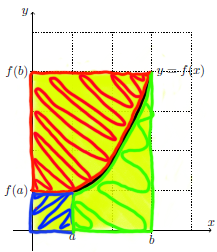
\includegraphics{highlighter.png}
    \end{figure}
    Now I will talk about the different aspects of the graph and why they are shaded a certain way. The yellow highlighted area is the area that returned with $bf(b)$. This is because it is a rectangle with sides of length $b$ and $f(b)$. The next term is $af(a)$. This term is the red shaded area. The area in the blue is the integral $\displaystyle{\int_{f(a)}^{f(b)}\!g(y)\,dy}$.
    The area in the green is the remaining area after subtracting the blue and the red from the yellow area. This area is equivalent to $\displaystyle{\int_a^b\!f(x)\,dx}$ which shows that $(b)$ is correct geometrically.
\end{enumerate}
\begin{center}
    Professional Problem on Page 6. $\rightarrow$
\end{center}


\newpage


\item \textbf{Professional Problem:}
\begin{enumerate}
    \item Use the reduction formula to show that $\int_{-\pi}^{\pi}\!\sin^nx\,dx=\dfrac{n-1}{n}\int_{-\pi}^{\pi}\sin^{n-2}x\,dx$.
    \item Use part $(a)$ to evaluate $\int_{-\pi}^{\pi}\sin^2x\,dx$.
    \item Use induction to prove $\int_{-\pi}^{\pi}\sin^{2n}x\,dx=\frac{(2n-1)...5\cdot3\cdot1}{(2n)...6\cdot4\cdot2}(2\pi)$.
\end{enumerate}

\begin{enumerate}
    
    \item The reduction formula is 
    \begin{align*}
        \int\!\sin^nx\,dx&=-\frac{1}{n}\cos x\sin^{n-1}x+\frac{n-1}{n}\int\!\sin^{n-2}x\,dx
    \end{align*}
    Using the Evaluation Theorem, we can use it on the reduction formula and simplify. This results in an expression like
    \begin{align*}
        \left[-\frac{1}{n}\cos x\sin^{n-1}x+\frac{n-1}{n}\int\!\sin^{n-2}x\,dx\right]_{-\pi}^{\pi}&=\left[-\frac{1}{n}\cos x\sin^{n-1}x\right]_{\pi}^\pi+\left[\frac{n-1}{n}\int\!\sin^{n-2}x\,dx\right]_{-\pi}^\pi \\
        &=-\frac{\cos (-\pi)\sin^{n-1}(-\pi)}{n}+\frac{\cos \pi\sin^{n-1}\pi}{n}i+\frac{n-1}{n}\int_{-\pi}^{\pi}\!\sin^{n-2}x\,dx \\
        &=\frac{1}{n}\cdot0+\frac{1}{n}\cdot0+\frac{n-1}{n}\int_{-\pi}^{\pi}\!\sin^{n-2}x\,dx \\
        &=\frac{n-1}{n}\int_{-\pi}^{\pi}\!\sin^{n-2}x\,dx
    \end{align*}
    We have shown that $\int_{-\pi}^{\pi}\!\sin^nx\,dx=\dfrac{n-1}{n}\int_{-\pi}^{\pi}\sin^{n-2}x\,dx$.

    \item Part $(a)$ states that the power of the sine in the original integrand is equal to $n$. Therefore, a $\sin^2x$ in the integrand means $n=2$. We can now plug $n$ into the simplified reduction formula now to form the integral
    \[\frac{2-1}{2}\int_{-\pi}^{\pi}\!\sin^{2-2}x\,dx\]
    Simplifying this will form the expressions
    \begin{align*}
        \frac{1}{2}\int_{-\pi}^{\pi}\!\sin^{0}x\,dx &=\frac{1}{2}\int_{-\pi}^{\pi}\!1\,dx \\
        &=\frac{1}{2}\cdot\left(\pi-(-\pi)\right) \\
        &=\pi
    \end{align*}
    Simplifying has given us the answer $\pi$. The integral $\int_{-\pi}^{\pi}\sin^2x\,dx=\pi$.

    \item Let us start our proof by induction by setting out the base case where $n=1$. Solving this using the formula provides the solution,
    \begin{align*}
        \frac{1}{2}(2\pi)&=\pi
    \end{align*}
    We know this is true since we solved for $n=1$ in part $(b)$. For our induction hypothesis let us assume that the prior formula holds true for all $n=k$. If the equation is true for all $k+1$, then
    \begin{align}
        int_{-\pi}^{\pi}\sin^{2k+2}x\,dx&=\int_{-\pi}^{\pi}\sin^{2k}x\,dx\cdot\frac{2k+1}{2k+2}
    \end{align}
    If we use the equation we proved was true in part $(a)$, we can change the left hand side to
    \begin{align*}
        \frac{2k+2-1}{2k+2}\int_{-\pi}^{\pi}\sin^{2k+2-2}x\,dx&=\frac{2k+1}{2k+2}\int_{-\pi}^{\pi}\sin^{2k}x\,dx  
    \end{align*}
    Now that we have shown that both sides of equation (1) are equal, we have proved that $\int_{-\pi}^{\pi}\sin^{2n}x\,dx=\frac{(2n-1)...5\cdot3\cdot1}{(2n)...6\cdot4\cdot2}(2\pi)$.
    
\end{enumerate}
\end{enumerate}


\end{document}